\section{Mô-đun SyscallAD --- kiến trúc và thuật toán}
\label{sec:syscallad}

Đây là phần trọng tâm của báo cáo. SyscallAD là một mô-đun phát hiện bất thường
\emph{kết hợp}, biến luồng syscall thô thành các véc-tơ đặc trưng, chấm điểm bằng
tập hợp VAE\,+\,iForest và phát cờ khi điểm vượt ngưỡng. Mục này trình bày tuần tự
toàn bộ đường ống đó.

\subsection{Tổng quan đường ống phát hiện}
Luồng xử lý của SyscallAD gồm năm bước nối tiếp:
\[
\begin{aligned}
\text{luồng syscall} &\to \text{cửa sổ trượt} \to \text{trích đặc trưng}
\to \text{VAE\,+\,iForest}\\
&\to \text{hợp nhất \& ngưỡng} \to \text{cờ bất thường}.
\end{aligned}
\]
Mô hình được huấn luyện \emph{chỉ trên dữ liệu bình thường} (học một lớp), nên không
cần nhãn tấn công và có khả năng phát hiện cả mối đe dọa chưa từng thấy.
Hình~\ref{fig:pipeline} minh họa toàn bộ đường ống.

\begin{figure}[htbp]
  \centering
  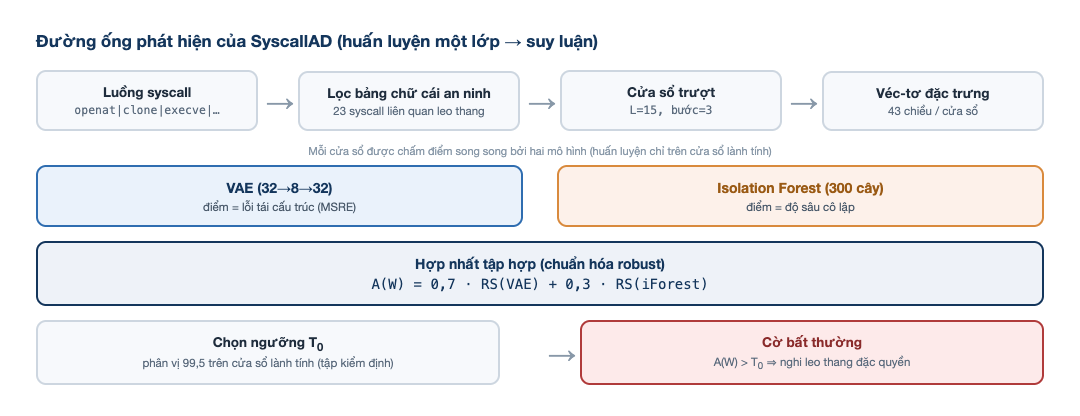
\includegraphics[width=\linewidth]{figures/syscallad-pipeline}
  \caption{Đường ống phát hiện của SyscallAD: lọc theo bảng chữ cái syscall an ninh
           $\to$ cửa sổ trượt $(15,3)$ $\to$ véc-tơ 43 chiều, chấm điểm song song bằng
           VAE (lỗi tái cấu trúc) và Isolation Forest (độ sâu cô lập), hợp nhất robust
           ($\alpha=0{,}7$), so với ngưỡng $T_0$ để phát cờ. Cả VAE và iForest đều
           huấn luyện \emph{chỉ trên cửa sổ lành tính}.}
  \label{fig:pipeline}
\end{figure}

\subsection{Thu thập, tiền xử lý và ``bảng chữ cái syscall an ninh''}
\label{subsec:alphabet}
SyscallAD đọc một chuỗi định danh syscall theo tiến trình. Một quyết định thiết kế
\emph{then chốt} là \textbf{bảng chữ cái syscall an ninh}: giới hạn không gian đặc
trưng về \textbf{23 syscall liên quan an ninh}---những lời gọi gắn với leo thang đặc
quyền và thoát container (\texttt{execve}, \texttt{clone},
\texttt{setuid/setgid/capset}, \texttt{openat}, \texttt{unlinkat},
\texttt{renameat2}, \texttt{mount}, \texttt{unshare}, \texttt{setns},
\texttt{pivot\_root}, \texttt{socket}, \texttt{connect}, \texttt{bind},
\texttt{mprotect}, \texttt{mmap}, \texttt{prctl}, \texttt{memfd\_create},
\texttt{splice}, \texttt{ptrace}, \texttt{init/finit\_module},
\texttt{bpf}---\emph{không} gồm các lời gọi mật độ cao read/write/close/futex). Đây
là một bước \emph{chọn lọc đặc trưng theo miền}: tập trung bộ phát hiện vào hành vi
đặc quyền và loại bớt nhiễu nền. Khâu huấn luyện lọc mỗi chuỗi DongTing về
\emph{đúng} tập này \emph{trước} khi cắt cửa sổ (xem hệ quả ở Mục~\ref{sec:results}).

\subsection{Trích đặc trưng theo cửa sổ trượt}
\label{subsec:fe}
Chuỗi syscall được cắt thành các \emph{cửa sổ trượt} chồng lấp (độ dài $L=15$, bước
nhảy $3$---giá trị mặc định theo công trình tham chiếu). Mỗi cửa sổ được biểu diễn
thành một véc-tơ \textbf{43 chiều} (Hình~\ref{fig:fe}):
\[
[\, \text{freq}_8 \mid \text{disc}_{15} \mid \text{stats}_8 \mid \text{cat}_{10}
   \mid \text{prefixspan}_2 \,].
\]
\begin{itemize}[leftmargin=1.6em]
  \item \textbf{freq (8):} tần suất trong cửa sổ của các syscall phổ biến trong bảng
        chữ cái.
  \item \textbf{disc (15):} \emph{hiện diện nhị phân} của các syscall đặc quyền hiếm
        (\texttt{ptrace}, \texttt{splice}, \texttt{unshare}, \texttt{setns},
        \texttt{mount}, \texttt{bpf}, \texttt{init/finit\_module}, \texttt{capset},
        \texttt{memfd\_create}\dots). Đây là \emph{tín hiệu cốt lõi cho leo thang
        đặc quyền} (Mục~\ref{sec:privesc}) và bền với pha loãng: một \texttt{ptrace}
        đơn lẻ vẫn bật bit dù lẫn giữa nhiều syscall thông thường.
  \item \textbf{stats (8):} entropy, số phần tử duy nhất, độ dài, tần suất lớn
        nhất\dots\ tóm tắt cấu trúc cửa sổ.
  \item \textbf{cat (10):} tần suất chuẩn hóa theo nhóm chức năng (tiến trình, tệp,
        bộ nhớ, mạng, tín hiệu, thời gian, IPC, an ninh, sự kiện I/O, khác)---``chữ
        ký hành vi'' theo danh mục.
  \item \textbf{prefixspan (2):} \texttt{[cờ-khớp, độ-dài-khớp/L]} từ việc đối sánh
        cửa sổ với một \emph{Cơ sở dữ liệu mẫu lành tính} (Mục~\ref{subsec:prefixspan}).
  \item \textbf{Đặc trưng thời gian} ($\Delta t$) bị \emph{tắt} vì DongTing
        (\texttt{strace -v -f}) không có dấu thời gian theo từng syscall
        (\texttt{has\_temporal=false}).
\end{itemize}
Chuẩn hóa bằng \texttt{RobustScaler} với phân vị $(1,99)$, \emph{chỉ} khớp trên cửa
sổ huấn luyện bình thường để tránh rò rỉ dữ liệu tấn công.

\begin{figure}[htbp]
  \centering
  
\includegraphics[width=\linewidth]{figures/feature-engineering}
  \caption{Kỹ thuật đặc trưng của SyscallAD: từ chuỗi syscall thô $\to$ lọc theo
           bảng chữ cái syscall an ninh $\to$ cửa sổ trượt $(15,3)$ $\to$ véc-tơ 43 chiều.}
  \label{fig:fe}
\end{figure}

\subsection{Cơ sở dữ liệu mẫu lành tính bằng PrefixSpan}
\label{subsec:prefixspan}
Để giảm dương tính giả, SyscallAD dùng PrefixSpan~\cite{prefixspan_pei}---một thuật
toán khai phá mẫu tuần tự---trên tập con \emph{lành tính} để rút ra các chuỗi con
syscall thường gặp, hợp lệ. Cơ sở dữ liệu mẫu này cho phép: (1) khớp sớm các cửa sổ
``đã biết là tốt''; (2) bỏ qua chấm điểm sâu cho cửa sổ khớp, giảm chi phí; (3) cung
cấp khả năng truy xuất ngữ nghĩa cho quyết định. Kết quả khớp được mã hóa thành hai
đặc trưng \texttt{prefixspan} ở trên.

\subsection{Mô hình thành phần}
\paragraph{Bộ mã hóa biến phân (VAE).}
Kiến trúc encoder--decoder ($32 \to 8 \to 32$), \texttt{hidden\_dim}=32,
\texttt{latent\_dim}=8, huấn luyện \emph{chỉ} trên cửa sổ bình thường bằng cách tối
thiểu hóa lỗi tái cấu trúc (MSRE). Điểm bất thường là MSRE; cửa sổ lệch phân phối
bình thường có MSRE lớn. Để xử lý hiện tượng \emph{sụp đổ hậu nghiệm} (posterior
collapse), VAE được huấn luyện đa hạt giống (seed 0,1,2) và giữ hạt giống có AUC
kiểm định tốt nhất.

\paragraph{Rừng cô lập (iForest).}
300 cây, \texttt{contamination}=0{,}02, cũng huấn luyện trên dữ liệu bình thường.
iForest cho điểm cao với các cửa sổ \emph{hiếm về mặt thống kê} mà VAE có thể bỏ
sót.

\subsection{Hợp nhất tập hợp}
Điểm cuối cho mỗi cửa sổ $W_i$ là tổ hợp tuyến tính có trọng số của hai điểm thành
phần (đã chuẩn hóa robust):
\begin{equation}
  A(W_i) = \alpha \cdot \mathrm{RS}\!\big(A_\text{VAE}(W_i)\big)
         + (1-\alpha)\cdot \mathrm{RS}\!\big(A_\text{iForest}(W_i)\big),
  \qquad \alpha = 0{,}7.
  \label{eq:ensemble}
\end{equation}
Trọng số $\alpha=0{,}7$ ưu tiên VAE; theo công trình tham chiếu, giá trị này được
chọn qua phân tích độ nhạy trên $\alpha \in \{0;0{,}25;0{,}5;0{,}7;0{,}85;1\}$.

\subsection{Chọn ngưỡng}
\label{subsec:threshold}
Biến quyết định để gắn cờ là \emph{điểm hợp nhất} $A(W_i)$ ở
phương trình~\eqref{eq:ensemble}, nên mọi ngưỡng dưới đây đều áp lên $A$ (không
phải lên riêng lỗi tái cấu trúc của VAE). Báo cáo phân biệt hai khái niệm ngưỡng:
\begin{itemize}[leftmargin=1.6em]
  \item \textbf{Ngưỡng ngoại tuyến $T_0$ (không rò rỉ):} chọn \emph{chỉ} trên tập
        kiểm định từ phân phối điểm $A$ của cửa sổ lành tính (mặc định:
        phân vị $99{,}5$, tương ứng định hướng ưu tiên precision của công trình tham
        chiếu); tập kiểm tra \emph{không} tham gia chọn ngưỡng. Đây là ngưỡng được
        dùng cho mọi kết quả trong báo cáo.
  \item \textbf{Ngưỡng động EMA (theo DeSFAM):} công trình tham chiếu cập nhật ngưỡng
        liên tục bằng Trung bình động hàm mũ. Báo cáo trình bày cơ chế này để đầy đủ,
        nhưng phần tái lập dùng ngưỡng cố định để dễ đối chiếu:
\end{itemize}
\begin{equation}
  T_{t+1} = \max\!\big(T_{\min},\; \beta T_t + (1-\beta) A(W_i)\big),
  \quad \beta=0{,}9,\; T_{\min}\ \text{là chặn dưới.}
  \label{eq:ema}
\end{equation}

\subsection{Thuật toán phát hiện}
Toàn bộ đường ống suy luận được tóm tắt trong Thuật toán~\ref{alg:syscallad}.

\begin{algorithm}[htbp]
\caption{Phát hiện bất thường syscall thời gian thực (SyscallAD)}
\label{alg:syscallad}
\KwIn{luồng syscall; VAE và iForest đã huấn luyện; bộ chuẩn hóa; ngưỡng $T_0$}
\KwOut{cờ bất thường cho mỗi cửa sổ}
khởi tạo cửa sổ trượt $W \gets \emptyset$;\quad $T \gets T_0$\;
\While{luồng syscall còn hoạt động}{
  thu syscall $s_t$ tại thời điểm $t$\;
  lọc theo bảng chữ cái syscall an ninh; thêm $s_t$ vào $W$\;
  \If{$W$ đã đầy ($|W| = L$)}{
    $f \gets \textsc{TrichDacTrung}(W)$ \tcp*{véc-tơ 43 chiều, đã chuẩn hóa}
    $A_\text{VAE} \gets \textsc{LoiTaiCauTruc}(\text{VAE}, f)$\;
    $A_\text{iForest} \gets \textsc{DiemCoLap}(\text{iForest}, f)$\;
    $A \gets 0{,}7\cdot \mathrm{RS}(A_\text{VAE}) + 0{,}3\cdot \mathrm{RS}(A_\text{iForest})$\;
    \eIf{$A > T$}{
      gắn cờ $W$ là bất thường; chuyển cho Mô-đun~3 (ngoài phạm vi)\;
    }{
      cập nhật ngưỡng động: $T \gets \max(T_{\min},\, \beta T + (1-\beta)A)$\;
    }
    trượt $W$ về phía trước theo bước nhảy\;
  }
}
\end{algorithm}
